\documentclass[11pt]{article}
\usepackage{geometry} 
\geometry{a4paper,top=3cm,bottom=3cm,left=2.5cm,right=2.5cm}   
\usepackage{multicol}
\usepackage[english, italian]{babel}
\usepackage{fancyhdr}
\usepackage{musicography}
\geometry{centering}
\usepackage{graphicx}


\pagestyle{fancy}                                 %serve ad inserire la linea sopra e il titolino
\rhead{\textsf{Lezione 4 "\textit{fondamenti dell'audio digitale 3}"}}
\renewcommand{\headrulewidth}{5pt} %grandezza della linea in alto
\renewcommand{\footrulewidth}{1pt}   % grandezza della linea in basso


\begin{document}
\begin{minipage}{0.55\linewidth}
\vspace{0.3cm}
{\large{\textbf{\textsf{Gabriele Petrillo}}}}\\\end{minipage}

\vspace{0.3cm}
\begin{minipage}{0.95\linewidth}
\begin{center}
{\huge{\textbf{\textsf{Fondamenti dell'audio digitale 2}}}} \\
\end{center}
\end{minipage}
\vspace*{0.2cm}


%=========ABSTRACT=======================
\begin{center}
\begin{minipage}[c]{14cm}
\begin{textit}

Ciò che segue è stato sviluppato a partire dalla dispensa di composizione del 09/12/2019 del prof. N.Bernardini presso il conservatorio S.Cecilia di Roma che possono essere consultati presso https://github.com/SMERM/TR-2019-2020/tree/master/A.A.2019-2020/COME-02/20191216. Questa dispensa tratta dell'implementazione in Octave di funzioni chirp e la fase di un segnale.

\end{textit}
\end{minipage}
\end{center}
\vspace*{0.2cm}

%=========ARTICOLO========================

\begin{multicols*}{2}
\parskip=0pt

\textbf{\textsf {Ex. 1 creare un glissando cosinusoidale}}\\

\noindent Con il termine \textit {chirp} si indica un segnale la cui frequenza aumenta o diminuisce nel tempo. Il termine è usato come sinonimo di \textit {sweep}.

Una sinusoide è definita come:
\[
f(t)=A*sin(2\pi ft + \phi)
\]

In un glissato lineare la frequenza istantanea $f(t)$ varia in modo lineare secondo la formula:

\[
f(t)=ct + f_0
\]

Dove $f_0$ è la frequenza al punto $t=0$, e $c$ è la costante del glissato secondo la formula:

\[
c = \frac{f_1 - f_0}{T}
\]

Dove $f_1$ è la frequenza di arrivo, $f_0$ è la frequenza di partenza e $T$ è il tempo del glissando.
La frequenza la possiamo descrivere come la derivata prima della fase, sarà necessario integrare nel tempo ottenendo questo risultato:

\[
x(t) = sin \Bigl [\phi_0 + 2\pi \Bigl(\frac{c}{2}t^2 + f_0t\Bigl) \Bigl]
\]

Di seguito il codice in Octave che risulta abbastanza chiaro senza bisogno di ulteriori spiegazioni:

\begin{center}
\begin{minipage}[c]{6.2cm}
\begin{sffamily}
\scriptsize

fc = 16000;	\%freq. di campionamento\\
sinc = 1/fc; \%periodo di camp.\\
dur = 2;	\%durata in secondi\\
t = [0:sinc:dur-sinc]; \%asse x\\							

hzstart = 0; \%frequenza iniziale\\
hzend = 4000;\%frequenza finale\\
amp = 0.9;\%ampiezza del segnale\\

c = (hzend-hzstart)/dur;\%costante di chirp\\
phase0 = 0;\%fase iniziale\\
freqfun = (c/2)*(t**2) + (hzstart*t);\%integrale della frequenza\\

out1 = cos(2*pi*freqfun+phase0)*amp;\%funzione di chirp\\

plot(t,out1);\\
axis ([0 0.1 -1 1])\\
print("plot01.png");\\

audiowrite("glissato.wav",out1,fc)

\end{sffamily}
\end{minipage}
\end{center}

lo script stampa il seguente plot

\begin{center}
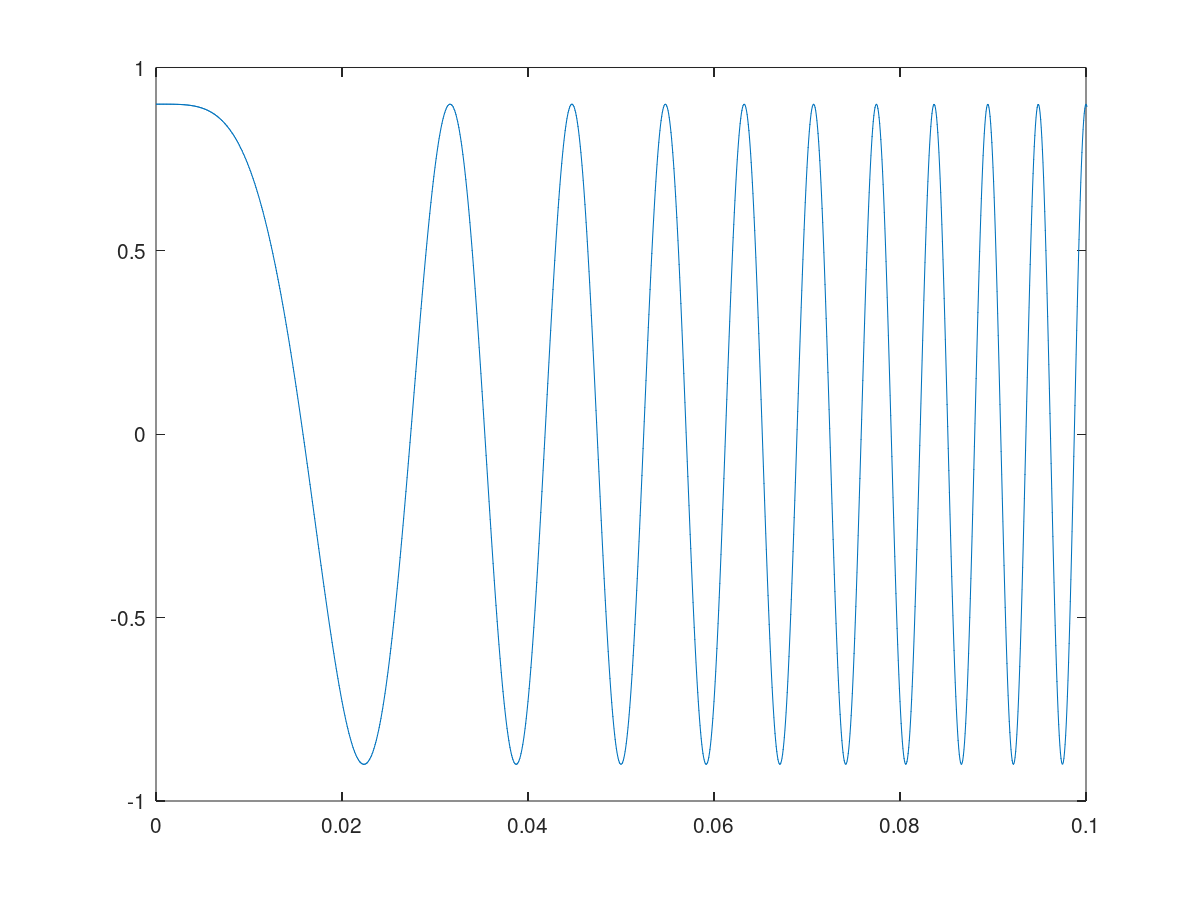
\includegraphics[scale=0.2]{images/plot01.png}

{\scriptsize \emph{fig.1 }}
\end{center}


\textbf{\textsf {Ia Fase}}\\

\noindent La formula di una sinusoide generica è:

\[
y(t) = Asin(2\pi ft)
\]

Dove $A$ è l'ampiezza del segnale sinusoidale, $2\pi f$ è la frequenza di oscillazione e $t$ è il tempo. Normalmente possiamo sostituire la funzione $sin$ con $cos$, quello che otteniamo è una funzione identica ma che parte da un punto diverso nell'istante $t = 0$. Visto che la posizione di $t = 0$ è arbitraria, non c'è nessuan differenza tra le due funzioni.

Tuttavia la distinzione fra seno e coseno può invece aver senso quando si devono confrontare fra loro due o più segnali sinusoidali. Si consideri per esempio la situazione in figura \textit{(fig2)}:

\begin{center}
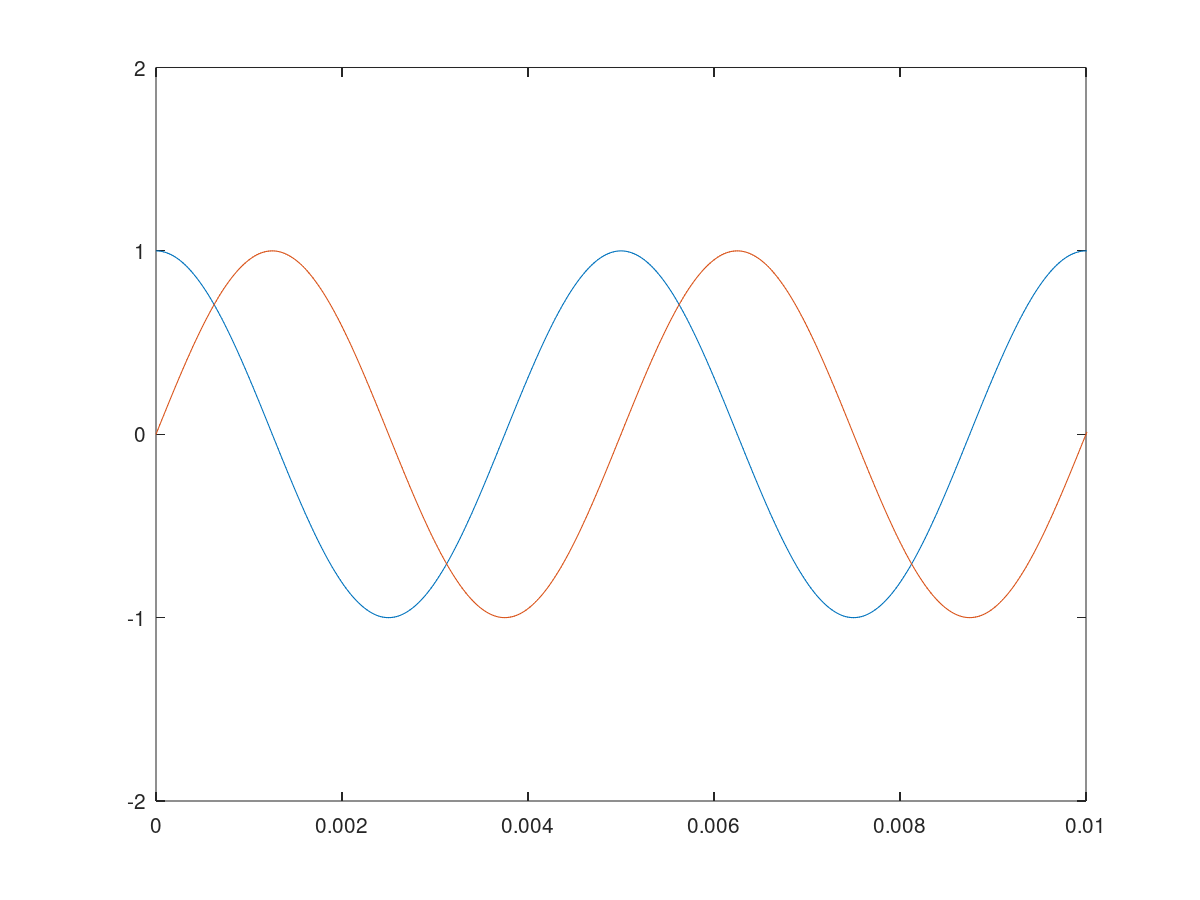
\includegraphics[scale=0.2]{images/plot02.png}

{\scriptsize \emph{fig.2 }}
\end{center}

Possiamo osservare che, quando $y_1(t)$ raggiunge i valori massimi, $y_2(t)$ passa per lo zero in modo decrescente, quello che cambia è quindi la posizione istantanea dell'onda, ovvero la \textit {fase} $\phi$ che è un parametro di un segnale sinusoidale che si misura in radianti e che rappresenta la traslazione di una sinusoide rispetto a un'altra:

\[
y(t) = Asin(2\pi ft + \phi)
\]

E' possibile visualizzare geometricamente il concetto di sfasamento fra due sinusoidi isofrequenziali pensando a due fasori(o vettori) in rotazione con la stessa velocità angolare $\omega$. La fase $\phi$ rappresenta l'angolo (costante) formato fra i due vettori:

\begin{center}
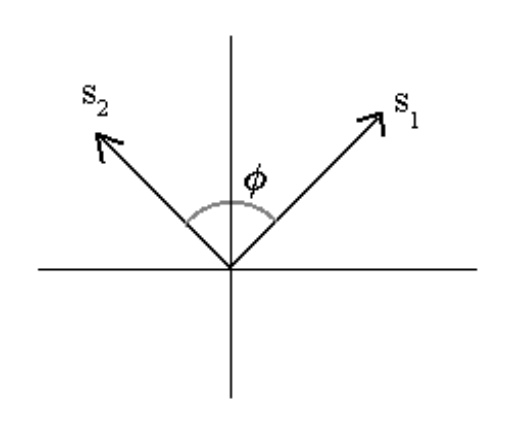
\includegraphics[scale=0.5]{images/plot03.png}

{\scriptsize \emph{fig.3 }}
\end{center}

Quindi possiamo pensare la fase come la combinazione di due angoli, infatti applicando le formule per la soma di due angoli:

\[
cos(\alpha + \beta) = cos(\alpha) cos (\beta) - sin(\alpha) sin(\beta)
\]

possiamo verificare che:

\[
y(t) = Asin(\omega t + \phi)
\]

 è equivalente a  
 
 \[
 y(t)=cos(\omega t) cos (\phi) - sin(\omega t) sin(\phi)
\]

Lo possiamo verificare in Octave con il seguente script:

\begin{center}
\begin{minipage}[c]{6.2cm}
\begin{sffamily}
\scriptsize

fc = 20000;\\
dur = 0.2;\\
sinc = 1/fc;\\

t = [0: sinc: dur-sinc];\\

fase = 0;\\
freq = 100;\\

y1 = cos(freq*2*pi*t+fase);\\
y2 = cos(fase)*cos(freq*2*pi*t)-sin(fase)*sin(freq*2*pi*t);\\ 

subplot(2,1,1)\\
plot(t,y1)\\

subplot(2,1,2)\\
plot(t,y2)\\

\end{sffamily}
\end{minipage}
\end{center}

\begin{center}
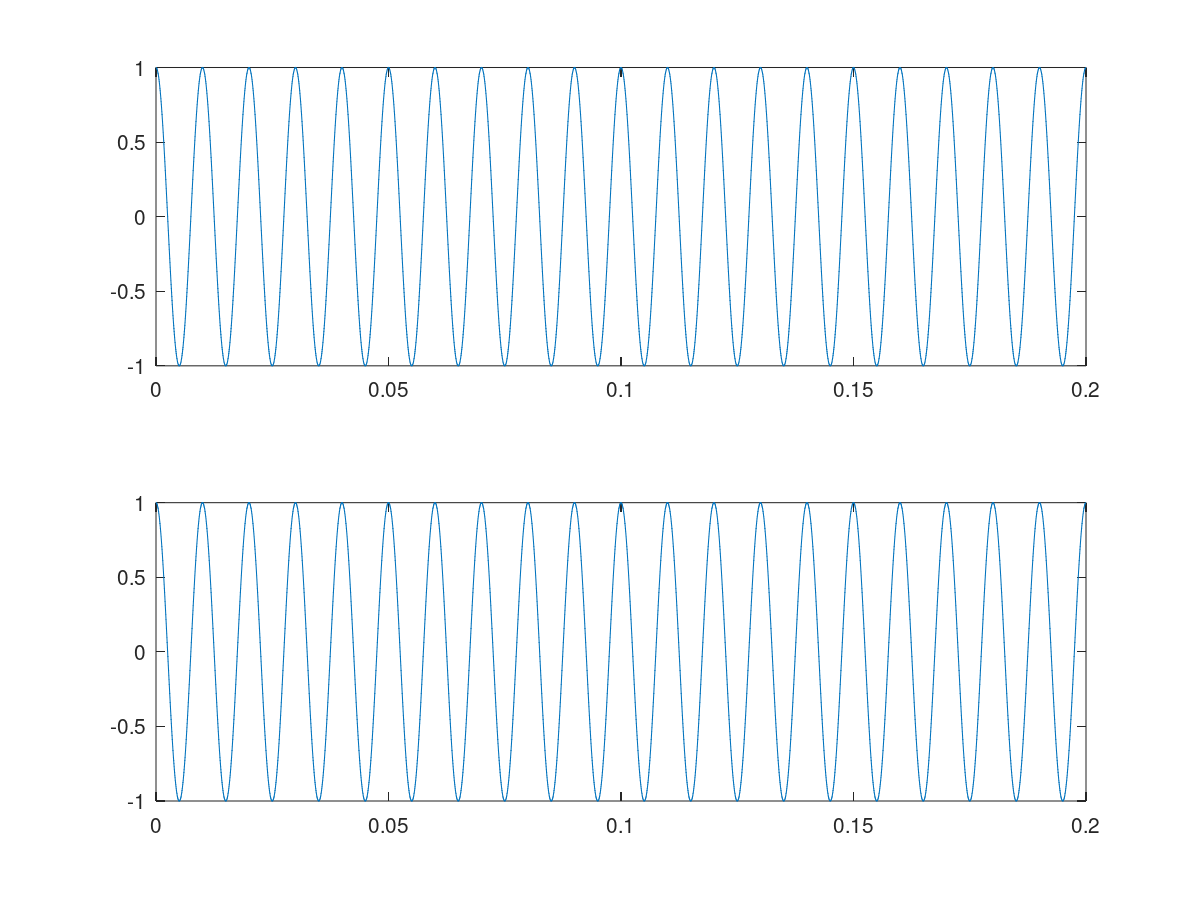
\includegraphics[scale=0.2]{images/plot04.png}

{\scriptsize \emph{fig.3 }}
\end{center}

Come possiamo vedere da \textit {fig.3} la fase delle due cosinusoidi è identica.

\section*{\centering\small{BIBLIOGRAFIA}}
•\textsc{\textsf {Santoboni, Riccardo e A.Rita, Ticari}}, \emph{Istituzioni di fisica acustica con elementi di psicoacustica. Per il musicista}, Papageno 2005\\

\end{multicols*}

\end{document}